\documentclass[../final_report.tex]{subfiles}
\usepackage{subfiles}
\usepackage{diagbox}
\graphicspath{{../../Lab5/plots/}}
\begin{document}

Αντικείμενο μελέτης της συγκεκριμένης άσκησης ήταν η εκτέλεση του αλγορίθμου K-means σε αρχιτεκτονική GPU.
Μελετάμε διαφορετικές τεχνικές με τις οποίες μπορούμε να δομήσουμε ένα πρόγραμμα που θα εκτελεστεί σε GPU και πως
μπορούμε να αξιοποιήσουμε όλο το υλικό για να μειώσουμε τον χρόνο εκτέλεσης, κρατώντας την GPU συνεχώς busy.

\subsubsection*{Σύντομη Παρουσίαση Υλικού - Αναφορά στο μοντέλο εκτέλεσης SIMT}

Τρέχοντας query μέσω του NVIDIA System Management Interface (nvidia - smi), αναγνωρίζουμε ότι η κάρτα γραφικών που
χρησιμοποιούμε για να τρέξουμε τα προγράμματα είναι η NVIDIA Tesla K40c.

\subsection{Τεχνικές υλοποίησης αλγορίθμων που εκτελούνται σε αρχιτεκτονικές GPU}

Στον προγραμματισμό με χρήση επιταχυντών, ο κλασσικός επεξεργαστής συνεχίζει να εκτελεί σημαντικό έργο, αρχικοποιώντας
και μεταφέροντας δεδομένα.

Ο χρόνος σειριακής εκτέλεσης για configuration \{Size, Coords, Clusters, Loops\} = \{256, 2, 16, 10\} είναι ίσος με 18446.2ms.
Για configuration \{Size, Coords, Clusters, Loops\} = \{256, 16, 16, 10\} είναι ίσος με 5484.8ms.

\textbf{Σημείωση:} Όλος ο κώδικας της άσκησης βρίσκεται σε ξεχωριστό .zip αρχείο στο Helios της ομάδας.


\subsection{K-Means Naive}
Η πρώτη υλοποίηση είναι και η πιο απλοϊκή σε σκέψη. Δρομολογούμε όσα νήματα όσα και τα στοιχεία του πίνακα στον οποίο εκτελούμε
τον αλγόριθμο K-means. Κάθε νήμα, με συγκεκριμένο thread ID, βρίσκει την κοντινότερη απόσταση από κάποιο κέντρο καλώντας την συνάρτηση euclid\_dist\_2.
Τέλος, αυξάνουμε το μέγεθος membership του κέντρου αυτού.

Οι διαστάσεις του πίνακα objects, είναι αριθμός\_αντικειμένων x αριθμός\_συντεταγμένων. 

Εφόσον τα warps, δηλαδή οι ομάδες των νημάτων, είναι πολλαπλάσια των 32, κάνουμε έναν έλεγχο ορίων ώστε αν δρομολογηθούν νήματα με 
thread ID μεγαλύτερο από τον αριθμό των αντικειμένων στον πίνακα, να μην δράσουν ώστε να μην επιχειρήσουν να αναζητήσουν στοιχείο σε 
διεύθυνση μνήμης που δεν έχει γίνει allocated.

Μεταξύ κάθε iteration, μεταφέρουμε από την CPU στην GPU τους πίνακες των κέτρων (Clusters) και από την GPU στην CPU τον πίνακα
membership, ώστε να γίνει η ανανέωση των κέτρων των cluster. Η CPU αναλαμβάνει την ανανέωση αυτή.

\subsubsection*{K-Means Naive - Αποτελέσματα}

\begin{figure}[H]
    \centering
    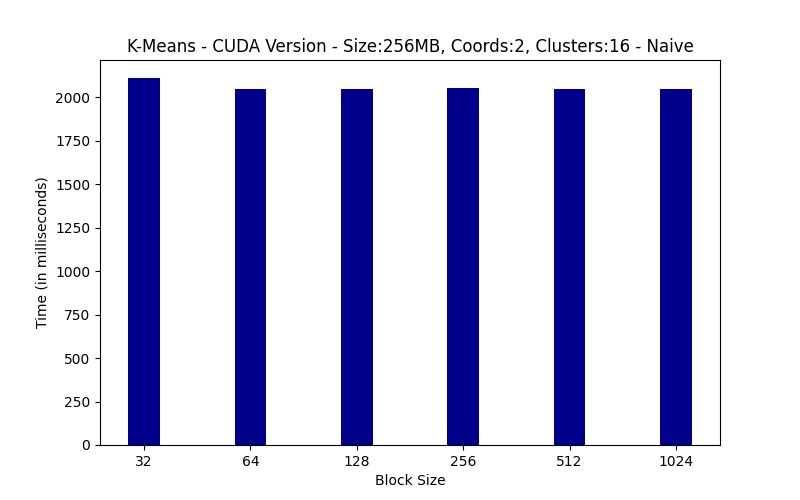
\includegraphics[scale=0.40]{/outFiles/plots/kmeans_gpu_Naive_2_time.jpg}
    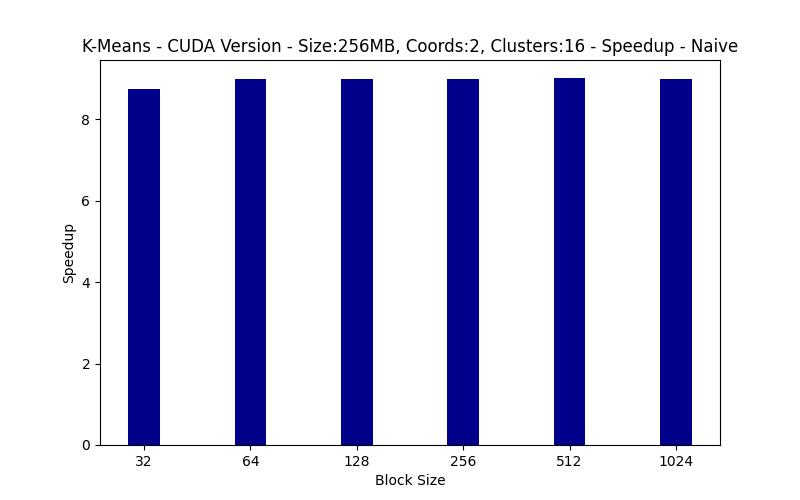
\includegraphics[scale=0.40]{/outFiles/plots/kmeans_gpu_Naive_2_speedup.jpg}
    \caption{K-Means Naive - GPU Edition}
    \label{fig:K-Means Naive - GPU Edition}
\end{figure}

\subsubsection*{K-Means Naive - Συμπεράσματα}

Η επίδοση της παράλληλης έκδοσης είναι εμφανώς καλύτερη από την σειριακή. Δεδομένου την απλότητα της υλοποίησης, το speedup
είναι αρκετά αξιοσημείωτο. Περαιτέρω, οι παράλληλες εκδόσεις με GPU έχουν το έξτρα overhead της μεταφοράς δεδομένων. Οι μετρήσεις
που κάναμε λαμβάνουν υπόψιν τους το φανόμενο αυτό, ώστε να είναι δίκαιη η σύγκριση με την σειριακή υλοποίηση.

Το block size δεν φαίνεται να επηρεάζει τα αποτελέσματα σε αυτή την υλοποίηση. 

% Εξήγησε γιατί όχι...

\subsubsection*{K-Means Naive - Best Time}

2051.098108ms - 128 Block Size

\subsection{K-Means Transpose}
Η υλοποίηση αυτή είναι ίδια με την σημαντική διαφορά ότι αλλάζουμε την λίστα των δεδομένων objects και clusters από row-based
σε column-based indexing. Ανανεώνουμε και την συνάρτηση εύρεσης απόστασης μεταξύ 2 σημείων σε column-based δεικτοδότηση.

\subsubsection*{K-Means Transpose - Αποτελέσματα}

\begin{figure}[H]
    \centering
    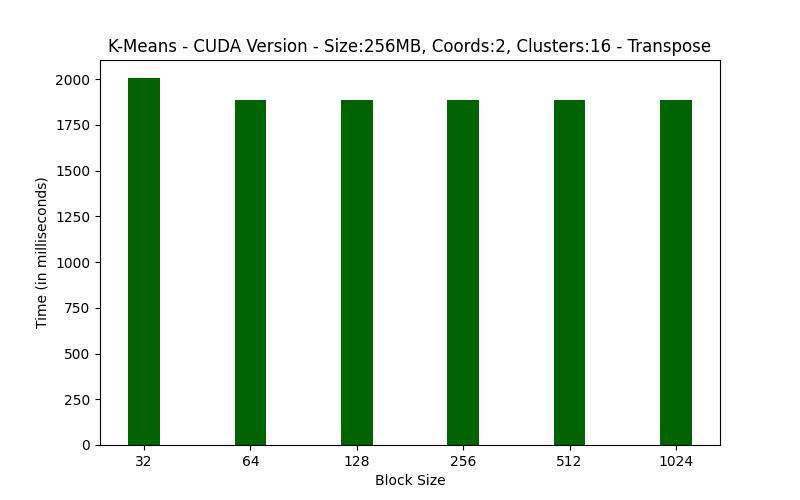
\includegraphics[scale=0.40]{/outFiles/plots/kmeans_gpu_Transpose_2_time.jpg}
    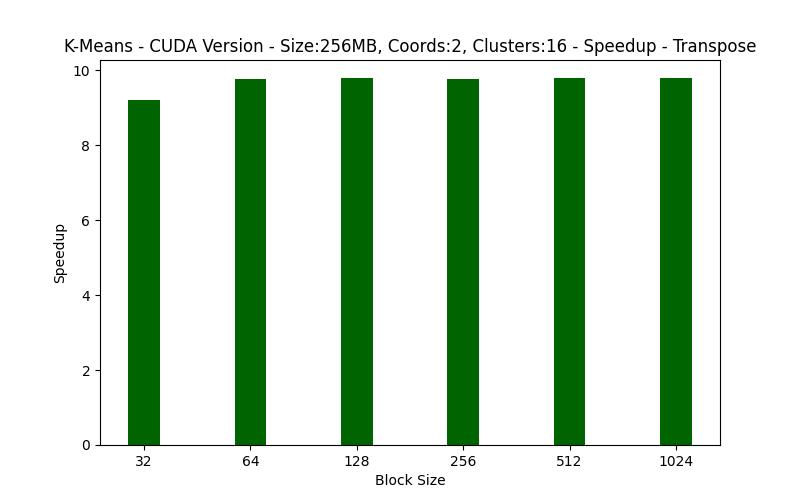
\includegraphics[scale=0.40]{/outFiles/plots/kmeans_gpu_Transpose_2_speedup.jpg}
    \caption{K-Means Transpose - GPU Edition}
    \label{fig:K-Means Transpose - GPU Edition}
\end{figure}

\subsubsection*{K-Means Transpose - Συμπεράσματα}

\subsubsection*{K-Means Transpose - Best Time}
1883.369207ms - 128 Block Size


\subsection{K-Means Shared Memory}
Το τελευταίο άμεσο βήμα βελτιστοποίησης είναι να εκμεταλευτούμε παραπάνω το ίδιο το υλικό. Οι \textbf{Streaming Multiprocessors} της κάρτας
γραφικών περιέχουν shared memory. Η ειδική αυτή μνήμη, δίνει την δυνατότητα στα νήματα να ... δεδομένα πιο γρήγορα. Στην υλοποίηση αυτή, τοποθετούμε
τον πίνακα cluster, δηλαδή τον πίνακα που περιέχει τις συντεταγμένες των κέτρων των cluster, στην διαμοιραζόμενη μνήμη. Η υπόλοιπη υλοποίηση
είναι ολόιδια με την Transpose.

\subsubsection*{K-Means Shared Memory - Αποτελέσματα}

\begin{figure}[H]
    \centering
    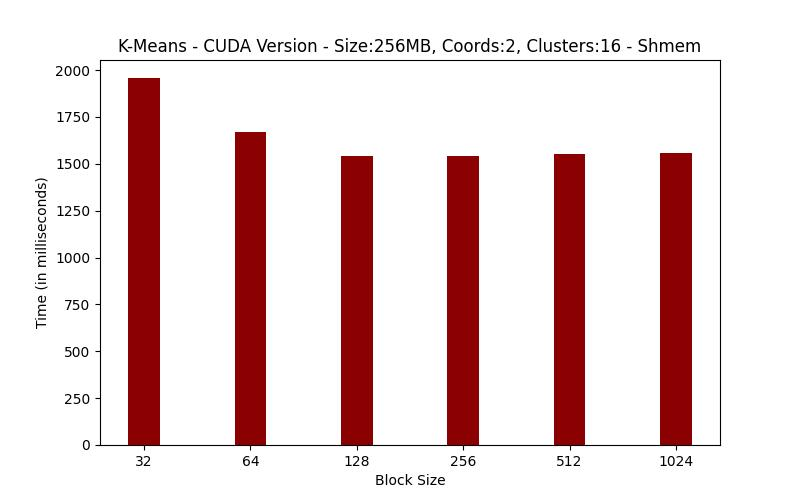
\includegraphics[scale=0.40]{/outFiles/plots/kmeans_gpu_Shmem_2_time.jpg}
    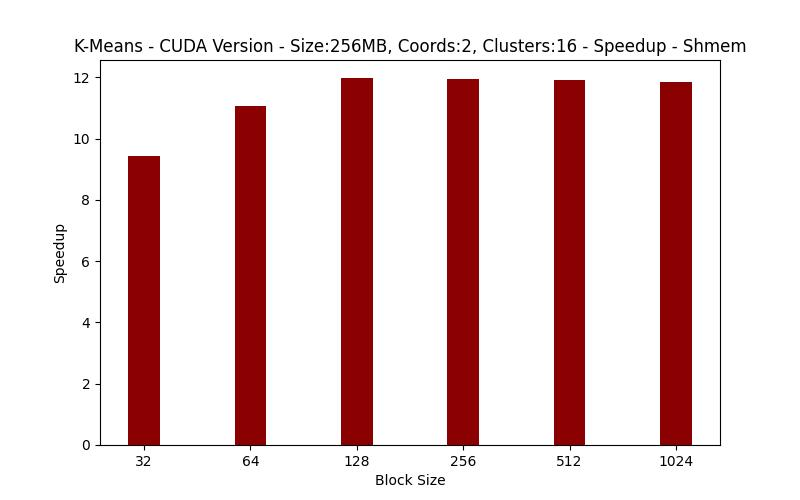
\includegraphics[scale=0.40]{/outFiles/plots/kmeans_gpu_Shmem_2_speedup.jpg}
    \caption{K-Means Shared - GPU Edition}
    \label{fig:K-Means Shared - GPU Edition}
\end{figure}

\subsubsection*{K-Means Shared Memory - Συμπεράσματα}

\subsubsection*{K-Means Shared Memory - Best Time}
1541.312933ms - 128 Block Size

\subsection{Σύγκριση υλοποιήσεων / bottleneck Analysis / μελέτη άλλων configuration}

\begin{figure}[H]
    \centering
    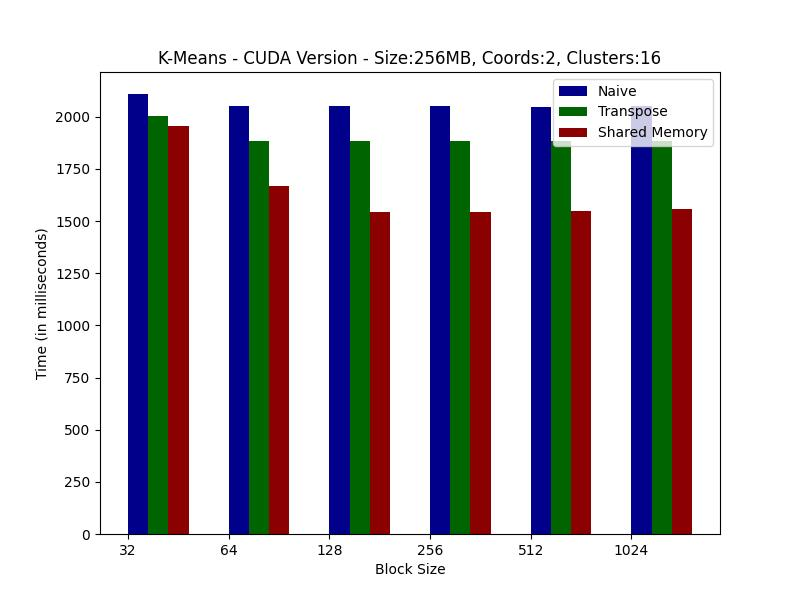
\includegraphics[scale=0.40]{/outFiles/plots/kmeans_gpu_common_figure_2_time.jpg}
    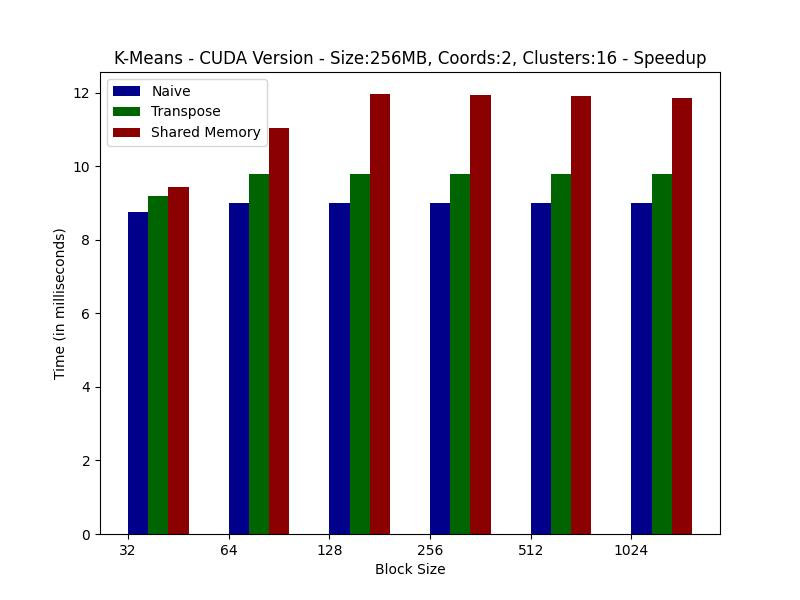
\includegraphics[scale=0.40]{/outFiles/plots/kmeans_gpu_common_figure_2_speedup.jpg}
    \caption{K-Means - GPU Edition Size - numCoords=2}
    \label{fig:K-Means - GPU Edition - {Size:256Mb, numCoords:2, numClusters:16}}
\end{figure}

\begin{figure}[H]
    \centering
    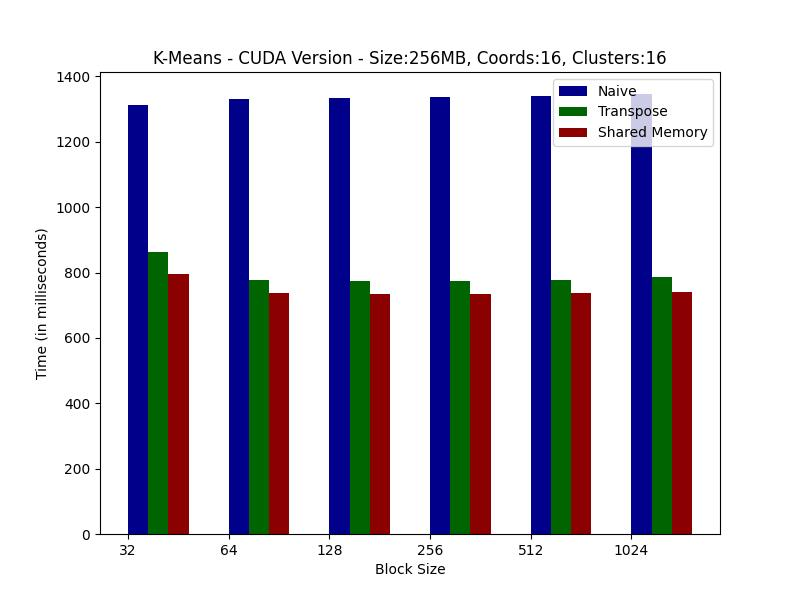
\includegraphics[scale=0.40]{/outFiles/plots/kmeans_gpu_common_figure_16_time.jpg}
    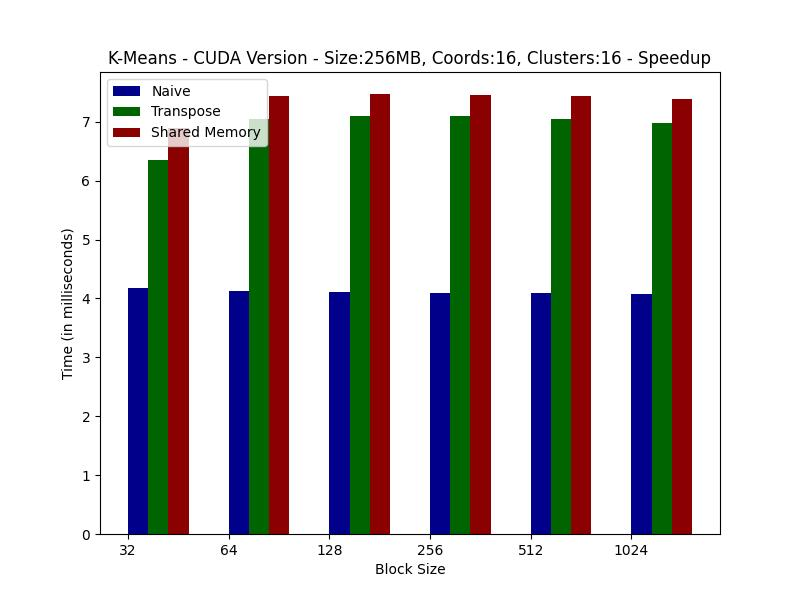
\includegraphics[scale=0.40]{/outFiles/plots/kmeans_gpu_common_figure_16_speedup.jpg}
    \caption{K-Means - GPU Edition Size - numCoords=16}
    \label{fig:K-Means - GPU Edition - {Size:256Mb, numCoords:16, numClusters:16}}
\end{figure}



\subsection{K-Means All GPU}
Ακόμα work in progress...


\end{document}